\documentclass[11pt,a4paper]{article}

% ============================================================================
% PACKAGES
% ============================================================================
\usepackage[utf8]{inputenc}
\usepackage[T1]{fontenc}
\usepackage{amsmath,amssymb,amsthm}
\usepackage{mathtools}
\usepackage{algorithm}
\usepackage{algpseudocode}
\usepackage{graphicx}
\usepackage{booktabs}
\usepackage{hyperref}
\usepackage{cleveref}
\usepackage{xcolor}
\usepackage{listings}
\usepackage{tikz}
\usetikzlibrary{arrows,shapes,positioning,calc,fit,backgrounds}
\usepackage{geometry}
\geometry{margin=1in}
\usepackage{natbib}
\usepackage{enumitem}
\usepackage{subcaption}
\usepackage{multirow}

% ============================================================================
% THEOREM ENVIRONMENTS
% ============================================================================
\theoremstyle{definition}
\newtheorem{definition}{Definition}[section]
\newtheorem{theorem}{Theorem}[section]
\newtheorem{lemma}[theorem]{Lemma}
\newtheorem{proposition}[theorem]{Proposition}
\newtheorem{corollary}[theorem]{Corollary}
\newtheorem{remark}{Remark}[section]

% ============================================================================
% CUSTOM COMMANDS
% ============================================================================
\newcommand{\dataset}{\mathcal{D}}
\newcommand{\query}{\mathbf{q}}
\newcommand{\score}{\text{score}}
\newcommand{\embed}{\phi}
\newcommand{\graph}{\mathcal{G}}
\newcommand{\nodes}{\mathcal{V}}
\newcommand{\edges}{\mathcal{E}}
\newcommand{\rel}{\text{rel}}
\newcommand{\confidence}{\gamma}
\newcommand{\evidence}{\mathcal{E}\text{vid}}
\newcommand{\fingerprint}{\mathbf{f}}
\newcommand{\compatibility}{\kappa}
\newcommand{\RRF}{\text{RRF}}
\newcommand{\BM}{\text{BM25}}
\newcommand{\NDCG}{\text{NDCG}}
\newcommand{\MRR}{\text{MRR}}
\newcommand{\sigmoid}{\sigma}

% Code listing style
\lstset{
    basicstyle=\ttfamily\small,
    keywordstyle=\color{blue},
    commentstyle=\color{gray},
    stringstyle=\color{orange},
    breaklines=true,
    frame=single,
    numbers=left,
    numberstyle=\tiny\color{gray}
}

% ============================================================================
% TITLE
% ============================================================================
\title{
    \textbf{Neural Search: Experiment-Aware Retrieval, Graph Reasoning, and Provenance for Reusable Neuroscience Datasets}\\[0.5em]
    \large A Scientific and Mathematical Foundation for Structured Scientific Discovery
}

\author{
    Neural Search Development Team\\
    \texttt{neural-search@research.org}
}

\date{May--June 2026}

\begin{document}

\maketitle

% ============================================================================
% ABSTRACT
% ============================================================================
\begin{abstract}
Neural Search is an experiment-aware discovery system for neural, behavioral, clinical, molecular, connectomics, and computational neuroscience datasets. Unlike generic document retrieval or chunk-based RAG systems, Neural Search treats datasets as structured scientific objects with typed metadata, ontological grounding, provenance tracking, and graph-based relational context. This whitepaper presents the mathematical foundations underlying the system, including information retrieval theory (BM25, vector space models, reciprocal rank fusion), knowledge graph theory (typed directed graphs, metapath reasoning, confidence propagation), representation learning (semantic fingerprints, field-specific embeddings), and evaluation methodology (NDCG, MRR, calibration). We formalize the hybrid scoring function, constraint satisfaction mechanics, and compatibility tensor that enable experiment-aware retrieval. Version 0.8 extends the system with \emph{latent usefulness scoring}: a 10-dimension intent-weighted scorer, graph-derived usefulness signals (affordance overlap, pipeline overlap, complementarity, PathSim hub-normalized metapath score), a graded NDCG evaluation framework with 4-level relevance labels, and an 8-variant ablation runner. The system achieves mean precision@5 of 76.7\%, label recall@10 of 87.8\%, MRR of 0.950, and NDCG@10 of 0.937 on benchmark queries while maintaining zero hard-negative violations.
\end{abstract}

\tableofcontents
\newpage

% ============================================================================
% SECTION 1: INTRODUCTION
% ============================================================================
\section{Introduction}
\label{sec:introduction}

\subsection{Motivation and Problem Statement}

The exponential growth of neuroscience datasets across repositories such as DANDI, OpenNeuro, Allen Brain Observatory, and NeMO Archive presents a fundamental discovery challenge. Researchers seeking datasets for replication, meta-analysis, or novel analysis face a search problem that traditional document retrieval cannot adequately address.

\begin{definition}[Scientific Dataset Search Problem]
Given a query $\query$ expressing experimental intent (tasks, modalities, species, analysis goals, constraints), retrieve a ranked list of datasets $\dataset_1, \dataset_2, \ldots, \dataset_k$ such that each $\dataset_i$ maximally satisfies the experimental requirements while providing sufficient metadata, quality assurance, and analysis affordances for scientific reuse.
\end{definition}

This problem differs fundamentally from web search or document retrieval:

\begin{enumerate}[label=(\roman*)]
    \item \textbf{Structured constraints}: A query like ``mouse Neuropixels decision-making data'' implicitly specifies organism (Mus musculus), recording modality (Neuropixels electrophysiology), and task ontology (decision-making behavioral paradigm).

    \item \textbf{Hard negatives}: Exclusions such as ``NOT EEG'' or ``without fMRI'' represent hard constraints, not soft preferences.

    \item \textbf{Analysis affordances}: Relevance depends not only on what data exists but whether it supports intended analyses (e.g., choice decoding, Q-learning modeling).

    \item \textbf{Provenance requirements}: Scientific reuse demands traceable evidence for metadata claims.
\end{enumerate}

\subsection{Thesis Statement}

The central thesis of Neural Search is that \textbf{neuroscience search should retrieve reusable experimental contexts, not just documents}. We formalize this through:

\begin{enumerate}
    \item \textbf{Dataset as experiment}: The object of search is a normalized dataset record with typed scientific structure.
    \item \textbf{Meaning as typed structure}: Scientific concepts are normalized into ontological categories.
    \item \textbf{Search as explanation}: Every result carries interpretable evidence.
    \item \textbf{Provenance as guardrail}: Assertions carry confidence and extraction lineage.
    \item \textbf{Benchmarks as compass}: Ranking changes are evaluated against reproducible metrics.
\end{enumerate}

% ============================================================================
% SECTION 2: MATHEMATICAL FOUNDATIONS
% ============================================================================
\section{Mathematical Foundations}
\label{sec:math-foundations}

\subsection{Information Retrieval Theory}

\subsubsection{Vector Space Model}

The Vector Space Model (VSM) represents documents and queries as vectors in a high-dimensional term space \citep{salton1975vector}.

\begin{definition}[Vector Space Representation]
Let $\mathcal{T} = \{t_1, t_2, \ldots, t_n\}$ be the vocabulary. A document $d$ is represented as:
\begin{equation}
    \mathbf{d} = (w_{1,d}, w_{2,d}, \ldots, w_{n,d}) \in \mathbb{R}^n
\end{equation}
where $w_{i,d}$ is the weight of term $t_i$ in document $d$.
\end{equation}
\end{definition}

The relevance between query $\query$ and document $d$ is computed via cosine similarity:
\begin{equation}
    \text{sim}(\query, \mathbf{d}) = \frac{\query \cdot \mathbf{d}}{\|\query\| \cdot \|\mathbf{d}\|} = \frac{\sum_{i=1}^n w_{i,q} \cdot w_{i,d}}{\sqrt{\sum_{i=1}^n w_{i,q}^2} \cdot \sqrt{\sum_{i=1}^n w_{i,d}^2}}
\end{equation}

\subsubsection{TF-IDF Weighting}

Term Frequency-Inverse Document Frequency (TF-IDF) balances term importance:

\begin{definition}[TF-IDF]
For term $t$ in document $d$ within corpus $\mathcal{C}$:
\begin{equation}
    \text{TF-IDF}(t, d, \mathcal{C}) = \text{TF}(t, d) \cdot \text{IDF}(t, \mathcal{C})
\end{equation}
where:
\begin{align}
    \text{TF}(t, d) &= \frac{f_{t,d}}{\max_{t' \in d} f_{t',d}} \quad \text{(normalized term frequency)} \\
    \text{IDF}(t, \mathcal{C}) &= \log \frac{|\mathcal{C}|}{|\{d \in \mathcal{C} : t \in d\}|} \quad \text{(inverse document frequency)}
\end{align}
\end{definition}

\subsubsection{BM25: Best Matching 25}

BM25 is a probabilistic relevance model that addresses TF-IDF limitations through saturation and length normalization \citep{robertson2009probabilistic}:

\begin{theorem}[BM25 Scoring Function]
\begin{equation}
    \BM(d, \query) = \sum_{t \in \query} \text{IDF}(t) \cdot \frac{f_{t,d} \cdot (k_1 + 1)}{f_{t,d} + k_1 \cdot \left(1 - b + b \cdot \frac{|d|}{\text{avgdl}}\right)}
\end{equation}
where:
\begin{itemize}
    \item $f_{t,d}$ is the frequency of term $t$ in document $d$
    \item $|d|$ is the document length
    \item $\text{avgdl}$ is the average document length in the corpus
    \item $k_1 \in [1.2, 2.0]$ controls term frequency saturation
    \item $b \in [0, 1]$ controls length normalization (typically $b = 0.75$)
\end{itemize}
\end{theorem}

The IDF component uses the Robertson-Sp\"arck Jones formula:
\begin{equation}
    \text{IDF}(t) = \log \frac{N - n_t + 0.5}{n_t + 0.5}
\end{equation}
where $N$ is the total number of documents and $n_t$ is the number containing term $t$.

\subsubsection{Field-Weighted BM25}

For structured scientific records, we extend BM25 to multiple fields:

\begin{definition}[Field-Weighted BM25]
Given fields $\mathcal{F} = \{f_1, f_2, \ldots, f_m\}$ with weights $\mathbf{w} = (w_1, \ldots, w_m)$:
\begin{equation}
    \BM_{\text{field}}(d, \query) = \sum_{f \in \mathcal{F}} w_f \cdot \BM(d_f, \query)
\end{equation}
where $d_f$ denotes the content of field $f$ in document $d$.
\end{definition}

In Neural Search, fields include: \texttt{title}, \texttt{description}, \texttt{tasks}, \texttt{modalities}, \texttt{species}, \texttt{brain\_regions}, \texttt{behavioral\_events}, \texttt{analysis\_goals}, and \texttt{standards}.

\subsection{Reciprocal Rank Fusion}

When combining multiple retrieval signals (lexical, semantic, graph-based), Reciprocal Rank Fusion (RRF) provides a robust aggregation method \citep{cormack2009reciprocal}:

\begin{definition}[Reciprocal Rank Fusion]
Given $m$ ranked lists $\{R_1, R_2, \ldots, R_m\}$, the RRF score for document $d$ is:
\begin{equation}
    \RRF(d) = \sum_{i=1}^m \frac{1}{k + \text{rank}_i(d)}
\end{equation}
where $\text{rank}_i(d)$ is the rank of $d$ in list $R_i$, and $k$ is a constant (typically $k = 60$) that mitigates the impact of high rankings.
\end{definition}

\begin{proposition}[RRF Properties]
RRF satisfies desirable fusion properties:
\begin{enumerate}
    \item \textbf{Rank-based}: Robust to score scale differences between rankers
    \item \textbf{Diminishing returns}: High ranks contribute more than low ranks
    \item \textbf{Consensus rewarding}: Documents ranked highly by multiple sources receive higher scores
\end{enumerate}
\end{proposition}

\subsection{Dense Retrieval and Embedding Spaces}

\subsubsection{Neural Embeddings}

Dense retrieval represents queries and documents in learned embedding spaces:

\begin{definition}[Bi-Encoder Architecture]
Given encoder $\embed: \mathcal{X} \rightarrow \mathbb{R}^d$, relevance is:
\begin{equation}
    \text{sim}(\query, d) = \embed(\query)^\top \embed(d)
\end{equation}
\end{definition}

\subsubsection{Semantic Fingerprints}

Neural Search extends single-vector embeddings to multi-aspect semantic fingerprints:

\begin{definition}[Semantic Fingerprint]
A dataset $d$ is represented as a concatenated multi-field embedding:
\begin{equation}
    \fingerprint(d) = \left[ \embed_{\text{text}}(d) \| \embed_{\text{task}}(d) \| \embed_{\text{mod}}(d) \| \embed_{\text{beh}}(d) \| \embed_{\text{ana}}(d) \| \embed_{\text{reg}}(d) \| \embed_{\text{des}}(d) \right]
\end{equation}
where $\|$ denotes concatenation and each $\embed_*$ encodes a specific semantic aspect.
\end{definition}

This factorization enables dimension-specific similarity:
\begin{equation}
    \text{sim}_{\text{aspect}}(d_i, d_j) = \frac{\embed_{\text{aspect}}(d_i) \cdot \embed_{\text{aspect}}(d_j)}{\|\embed_{\text{aspect}}(d_i)\| \cdot \|\embed_{\text{aspect}}(d_j)\|}
\end{equation}

% ============================================================================
% SECTION 3: KNOWLEDGE GRAPH THEORY
% ============================================================================
\section{Knowledge Graph Theory}
\label{sec:graph-theory}

\subsection{Typed Directed Graphs}

\begin{definition}[Scientific Knowledge Graph]
A scientific knowledge graph is a tuple $\graph = (\nodes, \edges, \tau_V, \tau_E, \evidence)$ where:
\begin{itemize}
    \item $\nodes$ is the set of nodes (datasets, papers, concepts, species, analyses)
    \item $\edges \subseteq \nodes \times \nodes$ is the set of directed edges
    \item $\tau_V: \nodes \rightarrow \mathcal{T}_V$ assigns node types from type set $\mathcal{T}_V$
    \item $\tau_E: \edges \rightarrow \mathcal{T}_E$ assigns edge types from relation set $\mathcal{T}_E$
    \item $\evidence: \nodes \cup \edges \rightarrow \mathcal{P}(\text{Evidence})$ maps elements to provenance evidence
\end{itemize}
\end{definition}

The Neural Search type system includes:
\begin{align*}
    \mathcal{T}_V &= \{\texttt{dataset}, \texttt{paper}, \texttt{task}, \texttt{modality}, \texttt{species}, \texttt{region}, \\
    &\quad\quad \texttt{event}, \texttt{analysis}, \texttt{standard}, \texttt{format}, \texttt{requirement}\} \\
    \mathcal{T}_E &= \{\texttt{has\_task}, \texttt{has\_modality}, \texttt{records\_region}, \texttt{has\_species}, \\
    &\quad\quad \texttt{uses\_standard}, \texttt{supports\_analysis}, \texttt{requires}, \texttt{linked\_to\_paper}\}
\end{align*}

\subsection{Provenance-Weighted Edges}

\begin{definition}[Edge Confidence]
Each edge $e \in \edges$ carries a confidence score:
\begin{equation}
    \confidence(e) = \sigma\left(\sum_{ev \in \evidence(e)} w_{\text{source}}(ev) \cdot w_{\text{method}}(ev)\right)
\end{equation}
where $\sigma$ is the sigmoid function, $w_{\text{source}}$ weights evidence source reliability, and $w_{\text{method}}$ weights extraction method confidence.
\end{definition}

Confidence propagates through paths:
\begin{equation}
    \confidence(\text{path}) = \prod_{e \in \text{path}} \confidence(e)
\end{equation}

\subsection{Metapath Theory}

Metapaths define semantically meaningful traversal patterns in heterogeneous graphs \citep{sun2011pathsim}:

\begin{definition}[Metapath]
A metapath $\mathcal{P}$ is a sequence of node types connected by edge types:
\begin{equation}
    \mathcal{P} = T_1 \xrightarrow{R_1} T_2 \xrightarrow{R_2} \cdots \xrightarrow{R_{l-1}} T_l
\end{equation}
\end{definition}

\begin{example}[Scientific Metapaths]
\begin{align*}
    \mathcal{P}_{\text{analysis}} &= \texttt{Dataset} \xrightarrow{\texttt{has\_event}} \texttt{Event} \xrightarrow{\texttt{required\_for}} \texttt{Analysis} \\
    \mathcal{P}_{\text{paper}} &= \texttt{Dataset} \xrightarrow{\texttt{linked\_to}} \texttt{Paper} \xrightarrow{\texttt{studies}} \texttt{Task} \\
    \mathcal{P}_{\text{similar}} &= \texttt{Dataset} \xrightarrow{\texttt{has\_task}} \texttt{Task} \xleftarrow{\texttt{has\_task}} \texttt{Dataset}
\end{align*}
\end{example}

\begin{definition}[Metapath-Based Similarity]
The PathSim similarity between nodes $v_i$ and $v_j$ along metapath $\mathcal{P}$ is:
\begin{equation}
    \text{PathSim}(v_i, v_j | \mathcal{P}) = \frac{2 \cdot |\text{paths}_\mathcal{P}(v_i, v_j)|}{|\text{paths}_\mathcal{P}(v_i, v_i)| + |\text{paths}_\mathcal{P}(v_j, v_j)|}
\end{equation}
\end{definition}

\subsection{Graph Neural Features}

Graph-derived features augment retrieval:

\begin{definition}[Node Centrality Features]
For node $v \in \nodes$:
\begin{align}
    \text{degree}(v) &= |\{u : (v, u) \in \edges \text{ or } (u, v) \in \edges\}| \\
    \text{PageRank}(v) &= \frac{1-d}{N} + d \sum_{u \in \text{in}(v)} \frac{\text{PageRank}(u)}{|\text{out}(u)|} \\
    \text{betweenness}(v) &= \sum_{s \neq v \neq t} \frac{\sigma_{st}(v)}{\sigma_{st}}
\end{align}
where $d$ is the damping factor, $\sigma_{st}$ is the number of shortest paths from $s$ to $t$, and $\sigma_{st}(v)$ is the number passing through $v$.
\end{definition}

% ============================================================================
% SECTION 4: HYBRID SCORING FORMALIZATION
% ============================================================================
\section{Hybrid Scoring Formalization}
\label{sec:scoring}

\subsection{Multi-Signal Scoring Function}

The Neural Search scoring function combines heterogeneous evidence:

\begin{theorem}[Hybrid Score]
For dataset $d$ and query $\query$, the relevance score is:
\begin{equation}
\begin{split}
    \score(d, \query) = \text{clamp}\Bigg(
        &w_{\text{task}} \cdot S_{\text{task}}(d, \query) + w_{\text{beh}} \cdot S_{\text{behavior}}(d, \query) \\
        &+ w_{\text{mod}} \cdot S_{\text{modality}}(d, \query) + w_{\text{aff}} \cdot S_{\text{affordance}}(d, \query) \\
        &+ w_{\text{meta}} \cdot S_{\text{metadata}}(d, \query) + w_{\text{sem}} \cdot S_{\text{semantic}}(d, \query) \\
        &+ w_{\text{field}} \cdot S_{\text{field}}(d, \query) + w_{\text{graph}} \cdot S_{\text{graph}}(d, \query) \\
        &+ w_{\text{ready}} \cdot S_{\text{readiness}}(d) + w_{\text{paper}} \cdot S_{\text{paper}}(d, \query) \\
        &- \lambda_{\text{mismatch}} \cdot P_{\text{mismatch}}(d, \query) \\
        &- \lambda_{\text{missing}} \cdot P_{\text{missing}}(d, \query) \\
        &- \lambda_{\text{hard}} \cdot P_{\text{hard\_negative}}(d, \query),
    \quad 0, 1\Bigg)
\end{split}
\end{equation}
where $\text{clamp}(x, a, b) = \max(a, \min(x, b))$.
\end{theorem}

\subsection{Component Score Functions}

\subsubsection{Ontology Matching Scores}

\begin{definition}[Set-Based Ontology Score]
For ontology-grounded fields (tasks, modalities, regions):
\begin{equation}
    S_{\text{onto}}(d, \query) = \frac{|L_d \cap L_\query|}{|L_\query|} \cdot \frac{1}{1 + \beta \cdot |L_d \setminus L_\query|}
\end{equation}
where $L_d$ is the label set of $d$, $L_\query$ is the query label set, and $\beta$ penalizes extraneous labels.
\end{definition}

With hierarchical ontologies, we use weighted Jaccard with ancestor expansion:
\begin{equation}
    S_{\text{hier}}(d, \query) = \frac{\sum_{l \in L_\query} \max_{l' \in L_d} \text{sim}_{\text{onto}}(l, l')}{|L_\query|}
\end{equation}

\subsubsection{Semantic Similarity Score}

\begin{equation}
    S_{\text{semantic}}(d, \query) = \frac{\embed(\query) \cdot \embed(d)}{\|\embed(\query)\| \cdot \|\embed(d)\|}
\end{equation}

\subsubsection{Field-Specific Semantic Score}

\begin{equation}
    S_{\text{field}}(d, \query) = \sum_{f \in \mathcal{F}} w_f \cdot \frac{\embed_f(\query) \cdot \embed_f(d)}{\|\embed_f(\query)\| \cdot \|\embed_f(d)\|}
\end{equation}

\subsubsection{Readiness Score}

Dataset readiness combines metadata completeness and quality indicators:
\begin{equation}
    S_{\text{readiness}}(d) = \alpha_1 \cdot \text{completeness}(d) + \alpha_2 \cdot \text{standardization}(d) + \alpha_3 \cdot \text{QA}(d)
\end{equation}

where:
\begin{align}
    \text{completeness}(d) &= \frac{|\text{populated\_fields}(d)|}{|\text{required\_fields}|} \\
    \text{standardization}(d) &= \mathbf{1}[d \text{ uses recognized standard}] \\
    \text{QA}(d) &= \text{quality\_assurance\_score}(d)
\end{align}

\subsection{Penalty Functions}

\subsubsection{Hard Negative Constraint Violation}

\begin{definition}[Hard Negative Penalty]
For excluded set $\mathcal{X}_\query$ (modalities, species, sources, etc.):
\begin{equation}
    P_{\text{hard\_negative}}(d, \query) =
    \begin{cases}
        +\infty & \text{if } L_d \cap \mathcal{X}_\query \neq \emptyset \\
        0 & \text{otherwise}
    \end{cases}
\end{equation}
\end{definition}

In practice, hard negatives are filtered before scoring, ensuring zero violations.

\subsubsection{Missing Required Metadata Penalty}

\begin{equation}
    P_{\text{missing}}(d, \query) = \sum_{r \in \text{required}(\query)} \mathbf{1}[\text{missing}(d, r)] \cdot w_r
\end{equation}

\subsection{Intent-Adaptive Weight Profiles}

Query intent determines weight profiles:

\begin{definition}[Intent Classification]
Let $\mathcal{I} = \{\texttt{lookup}, \texttt{task\_search}, \texttt{modality\_search}, \texttt{affordance\_search}, \texttt{similarity}, \texttt{exploration}\}$ be the intent space. The weight vector $\mathbf{w}_i$ varies by intent:
\end{definition}

\begin{table}[h]
\centering
\caption{Intent-Specific Weight Profiles}
\begin{tabular}{lcccccc}
\toprule
Weight & Lookup & Task & Modality & Affordance & Similarity & Exploration \\
\midrule
$w_{\text{task}}$ & 0.10 & \textbf{0.30} & 0.15 & 0.15 & 0.20 & 0.15 \\
$w_{\text{modality}}$ & 0.10 & 0.15 & \textbf{0.30} & 0.15 & 0.15 & 0.15 \\
$w_{\text{affordance}}$ & 0.05 & 0.15 & 0.10 & \textbf{0.35} & 0.10 & 0.10 \\
$w_{\text{semantic}}$ & 0.15 & 0.10 & 0.10 & 0.10 & \textbf{0.25} & 0.20 \\
$w_{\text{graph}}$ & 0.05 & 0.10 & 0.10 & 0.10 & 0.15 & \textbf{0.20} \\
\bottomrule
\end{tabular}
\end{table}

% ============================================================================
% SECTION 4b: LATENT USEFULNESS SCORING (v0.8)
% ============================================================================
\section{Latent Usefulness Scoring}
\label{sec:latent-usefulness}

\subsection{Motivation}

Relevance in scientific dataset search is intent-dependent. A dataset that perfectly matches a \emph{replication} query may be poorly suited for \emph{meta-analysis} even if both queries share surface-level keywords. Latent usefulness scoring formalizes this by defining seven researcher intents, scoring candidates along ten orthogonal dimensions, and weighting those dimensions per intent.

\subsection{Researcher Intent Taxonomy}

\begin{definition}[UsefulnessIntent]
Let $\mathcal{I}_U = \{I_1, \ldots, I_7\}$ be the researcher intent space:
\begin{align*}
    I_1 &= \texttt{STRICT\_LOOKUP} & &\text{(find exact dataset by ID/name)} \\
    I_2 &= \texttt{REPLICATION}    & &\text{(reproduce a specific experiment)} \\
    I_3 &= \texttt{META\_ANALYSIS} & &\text{(aggregate across multiple studies)} \\
    I_4 &= \texttt{PIPELINE\_REUSE}& &\text{(reuse existing analysis pipeline)} \\
    I_5 &= \texttt{CROSS\_DATASET\_COMPARISON} & &\text{(compare modalities or species)} \\
    I_6 &= \texttt{EXPLORATION}    & &\text{(discover datasets by topic)} \\
    I_7 &= \texttt{METHOD\_TRANSFER} & &\text{(apply method from one domain to another)}
\end{align*}
\end{definition}

Intent is classified rule-based via regex patterns and keyword heuristics with a confidence score $\gamma \in [0, 1]$.

\subsection{Ten-Dimension Usefulness Score}

\begin{definition}[DatasetContext]
A dataset candidate is represented as a context vector:
\begin{equation}
    C = (\text{modalities}, \text{tasks}, \text{species}, \text{regions}, \text{affordances}, \text{standards},
         N_s, N_t, N_u, b_{\text{ts}}, q)
\end{equation}
where $N_s, N_t, N_u$ are session/trial/subject counts, $b_{\text{ts}}$ indicates timestamp availability, and $q$ is a quality score.
\end{definition}

\begin{theorem}[Usefulness Score]
For query context $C_q$, candidate $C_d$, and intent $i \in \mathcal{I}_U$:
\begin{equation}
    U(C_q, C_d, i) = \sum_{k=1}^{10} w_k(i) \cdot s_k(C_q, C_d)
\end{equation}
where $\sum_k w_k(i) = 1$ for all $i$, and the ten dimension scores are:
\begin{align}
    s_1 &= \text{Jaccard}(\text{modalities}_q, \text{modalities}_d) & \text{(modality alignment)} \\
    s_2 &= \text{Jaccard}(\text{tasks}_q, \text{tasks}_d) & \text{(task alignment)} \\
    s_3 &= \text{Jaccard}(\text{species}_q, \text{species}_d) & \text{(species alignment)} \\
    s_4 &= \text{Jaccard}(\text{regions}_q, \text{regions}_d) & \text{(region alignment)} \\
    s_5 &= \text{Jaccard}(\text{affordances}_q, \text{affordances}_d) & \text{(affordance alignment)} \\
    s_6 &= \text{Jaccard}(\text{standards}_q, \text{standards}_d) & \text{(pipeline compatibility)} \\
    s_7 &= f_{\log}(N_s) & \text{(scale: sessions)} \\
    s_8 &= f_{\log}(N_t) & \text{(scale: trials)} \\
    s_9 &= \text{PathSim}(\cdot \mid \mathcal{G}) & \text{(graph proximity; falls back to 0.3 if graph unavailable, implemented v0.9)} \\
    s_{10} &= 0.0 & \text{(neural signature similarity, Phase-4 placeholder)}
\end{align}
\end{theorem}

The log-power scale function handles count fields with wide dynamic range:
\begin{equation}
    f_{\log}(n) = \begin{cases} 0.3 & n = 0 \text{ or None} \\ \min\!\left(1,\, \frac{\ln(1+n)}{\ln(1+10000)}\right) & \text{otherwise} \end{cases}
\end{equation}

Jaccard similarity uses a neutral prior for empty sets:
\begin{equation}
    \text{Jaccard}(A, B) = \begin{cases} 0.5 & A = B = \emptyset \\ 0 & A = \emptyset \text{ XOR } B = \emptyset \\ \frac{|A \cap B|}{|A \cup B|} & \text{otherwise} \end{cases}
\end{equation}

\subsection{Intent-Specific Weight Profiles}

\begin{table}[h]
\centering
\caption{Intent Weight Profiles ($w_k(i)$) — v0.8}
\small
\begin{tabular}{lrrrrrrr}
\toprule
Dimension & Lookup & Replication & Meta & Pipeline & Cross & Explore & Transfer \\
\midrule
Modality & 0.05 & 0.15 & 0.10 & 0.15 & 0.20 & 0.10 & 0.15 \\
Task     & 0.05 & 0.20 & 0.15 & 0.10 & 0.15 & 0.20 & 0.15 \\
Species  & 0.05 & 0.15 & 0.10 & 0.05 & 0.15 & 0.10 & 0.15 \\
Region   & 0.05 & 0.10 & 0.10 & 0.05 & 0.10 & 0.10 & 0.10 \\
Affordance & 0.05 & 0.05 & 0.15 & 0.20 & 0.10 & 0.15 & 0.15 \\
Standards & 0.05 & 0.05 & 0.05 & 0.20 & 0.05 & 0.05 & 0.05 \\
Scale-S  & 0.05 & 0.05 & 0.15 & 0.05 & 0.05 & 0.10 & 0.05 \\
Scale-T  & 0.05 & 0.05 & 0.10 & 0.05 & 0.05 & 0.05 & 0.05 \\
Graph    & 0.30 & 0.10 & 0.05 & 0.10 & 0.10 & 0.10 & 0.10 \\
Signature& 0.25 & 0.10 & 0.05 & 0.05 & 0.05 & 0.05 & 0.05 \\
\midrule
Sum      & 1.00 & 1.00 & 1.00 & 1.00 & 1.00 & 1.00 & 1.00 \\
\bottomrule
\end{tabular}
\end{table}

\subsection{Graph-Derived Usefulness Signals}

Four graph-derived signals augment the usefulness scorer:

\begin{definition}[Affordance Overlap]
\begin{equation}
    \text{aff\_overlap}(d_i, d_j) = \frac{|\text{affordances}(d_i) \cap \text{affordances}(d_j)|}{|\text{affordances}(d_i) \cup \text{affordances}(d_j)|}
\end{equation}
\end{definition}

\begin{definition}[Pipeline Overlap]
\begin{equation}
    \text{pipe\_overlap}(d_i, d_j) = \frac{|\text{standards}(d_i) \cap \text{standards}(d_j)|}{|\text{standards}(d_i) \cup \text{standards}(d_j)|}
\end{equation}
\end{definition}

\begin{definition}[Complementarity Score]
\begin{equation}
    \text{complement}(d_i, d_j) = 0.7 \cdot \frac{|A_i \triangle A_j|}{|A_i \cup A_j|} + 0.3 \cdot \frac{|A_i \cap A_j|}{|A_i \cup A_j|}
\end{equation}
where $A_k = \text{affordances}(d_k)$. High unique fractions reward complementary pairs; modest overlap rewards shared foundation.
\end{definition}

\begin{definition}[Hub-Normalized PathSim]
For metapath $\mathcal{P}$ and shared-neighbor sets $N_\mathcal{P}(\cdot)$ derived from the knowledge graph:
\begin{equation}
    \text{PathSim}_\mathcal{P}(d_i, d_j) = \frac{2 \cdot |N_\mathcal{P}(d_i) \cap N_\mathcal{P}(d_j)|}{|N_\mathcal{P}(d_i)| + |N_\mathcal{P}(d_j)|}
\end{equation}
The self-exclusion guard $\{v \neq \text{src}\}$ prevents hub nodes from inflating denominator terms.
\end{definition}

% ============================================================================
% SECTION 5: COMPATIBILITY TENSOR
% ============================================================================
\section{Dataset Compatibility Theory}
\label{sec:compatibility}

\subsection{Slot-Based Dataset Representation}

\begin{definition}[Experimental Slot Vector]
A dataset $d$ is represented as a slot vector:
\begin{equation}
    E(d) = \begin{pmatrix}
        \text{organism}(d) \\
        \text{taxon\_group}(d) \\
        \text{preparation}(d) \\
        \text{task\_family}(d) \\
        \text{task\_variant}(d) \\
        \text{event\_schema}(d) \\
        \text{modality\_family}(d) \\
        \text{device}(d) \\
        \text{signal\_type}(d) \\
        \text{brain\_region}(d) \\
        \text{region\_hierarchy}(d) \\
        \text{species\_homolog}(d) \\
        \text{data\_standard}(d) \\
        \text{file\_format}(d) \\
        \text{sampling\_resolution}(d) \\
        \text{analysis\_affordances}(d) \\
        \text{readiness}(d) \\
        \text{provenance\_confidence}(d)
    \end{pmatrix}
\end{equation}
\end{definition}

\subsection{Compatibility Function}

\begin{theorem}[Compatibility Score]
The compatibility between datasets $d_i$ and $d_j$ given query intent is:
\begin{equation}
\begin{split}
    \compatibility(d_i, d_j | \query) = &\sum_{k} w_k(\query) \cdot \text{match}_k(E_k(d_i), E_k(d_j)) \\
    &+ \lambda_g \cdot S_{\text{graph\_path}}(d_i, d_j) \\
    &+ \lambda_a \cdot S_{\text{analysis\_complement}}(d_i, d_j) \\
    &+ \lambda_p \cdot S_{\text{provenance\_agreement}}(d_i, d_j) \\
    &- \mu_c \cdot P_{\text{contradiction}}(d_i, d_j) \\
    &- \mu_m \cdot P_{\text{missing\_slot}}(d_i, d_j)
\end{split}
\end{equation}
\end{theorem}

\subsection{Compatibility Types}

\begin{definition}[Compatibility Categories]
We define five compatibility relations:

\begin{enumerate}
    \item \textbf{Equivalent context} ($\equiv$): Same or homologous task, modality, species, region, and event schema. Useful for replication and meta-analysis.
    \begin{equation}
        d_i \equiv d_j \iff \forall k \in \mathcal{K}_{\text{core}}: \text{match}_k(E_k(d_i), E_k(d_j)) > \theta_{\text{equiv}}
    \end{equation}

    \item \textbf{Complementary context} ($\oplus$): Same task but different modality, or same region but different species.
    \begin{equation}
        d_i \oplus d_j \iff \exists k_1, k_2: E_{k_1}(d_i) = E_{k_1}(d_j) \land E_{k_2}(d_i) \neq E_{k_2}(d_j)
    \end{equation}

    \item \textbf{Translational context} ($\rightarrow$): Cross-species mapping via homologous behaviors and regions.

    \item \textbf{Analysis-compatible} ($\sim_A$): Both satisfy requirements for analysis $A$.
    \begin{equation}
        d_i \sim_A d_j \iff \text{affordance}_A(d_i) = \text{affordance}_A(d_j) = \text{True}
    \end{equation}

    \item \textbf{Contrastive context} ($\bot$): Intentionally differ on one axis for controlled comparison.
\end{enumerate}
\end{definition}

% ============================================================================
% SECTION 6: ANALYSIS AFFORDANCES
% ============================================================================
\section{Analysis Affordance Theory}
\label{sec:affordances}

\subsection{Affordance as Constraint Satisfaction}

\begin{definition}[Analysis Affordance]
An analysis affordance $A$ is a predicate over dataset features:
\begin{equation}
    \text{affordance}_A(d) = \bigwedge_{r \in \text{requirements}(A)} \text{satisfies}(d, r)
\end{equation}
\end{definition}

\begin{example}[Choice Decoding Affordance]
\begin{equation}
    \text{affordance}_{\text{choice\_decoding}}(d) = \text{has\_neural}(d) \land \text{has\_choice\_labels}(d)
\end{equation}
\end{example}

\begin{example}[Q-Learning Modeling Affordance]
\begin{equation}
    \text{affordance}_{\text{Q-learning}}(d) = \text{has\_choice}(d) \land \text{has\_reward}(d) \land \text{has\_trial\_outcome}(d)
\end{equation}
\end{example}

\subsection{Hyperedge Requirements}

Some analyses require conjunctions that cannot be represented as simple edges:

\begin{definition}[Requirement Hyperedge]
A hyperedge $h = (A, \{r_1, \ldots, r_n\})$ represents that analysis $A$ requires \textit{all} of $r_1, \ldots, r_n$ simultaneously:
\begin{equation}
    \text{satisfies}(d, h) = \bigwedge_{i=1}^n \text{has\_feature}(d, r_i)
\end{equation}
\end{definition}

\subsection{Affordance Confidence}

\begin{equation}
    \confidence_A(d) = \prod_{r \in \text{requirements}(A)} \confidence(\text{evidence}(d, r))
\end{equation}

% ============================================================================
% SECTION 7: PROVENANCE AND CONFIDENCE
% ============================================================================
\section{Provenance and Confidence Modeling}
\label{sec:provenance}

\subsection{Evidence Labels}

\begin{definition}[Evidence Label]
An evidence label is a tuple:
\begin{equation}
    \ell = (\text{id}, \text{label}, \text{type}, \confidence, \text{evidence\_text}, \text{source\_field}, \text{extractor}, \text{version})
\end{equation}
\end{definition}

\subsection{Confidence Calibration}

Confidence scores should be calibrated such that:
\begin{equation}
    \mathbb{P}[\text{label correct} | \confidence = c] \approx c
\end{equation}

We measure calibration via reliability diagrams and Expected Calibration Error (ECE):
\begin{equation}
    \text{ECE} = \sum_{b=1}^B \frac{|B_b|}{N} \left| \text{acc}(B_b) - \text{conf}(B_b) \right|
\end{equation}
where $B_b$ are confidence bins, $\text{acc}(B_b)$ is accuracy within bin $b$, and $\text{conf}(B_b)$ is mean confidence.

\subsection{Confidence Source Hierarchy}

\begin{equation}
    \confidence_{\text{base}}(\ell) =
    \begin{cases}
        0.95 & \text{structured metadata field} \\
        0.85 & \text{curated synonym match} \\
        0.75 & \text{strong title pattern} \\
        0.60 & \text{description inference} \\
        0.40 & \text{path or filename evidence}
    \end{cases}
\end{equation}

% ============================================================================
% SECTION 8: EVALUATION METHODOLOGY
% ============================================================================
\section{Evaluation Methodology}
\label{sec:evaluation}

\subsection{Ranking Metrics}

\subsubsection{Precision at K}

\begin{definition}[Precision@K]
\begin{equation}
    P@K = \frac{|\text{relevant} \cap \text{top-}K|}{K}
\end{equation}
\end{definition}

\subsubsection{Recall at K}

\begin{definition}[Recall@K]
\begin{equation}
    R@K = \frac{|\text{relevant} \cap \text{top-}K|}{|\text{relevant}|}
\end{equation}
\end{definition}

\subsubsection{Mean Reciprocal Rank}

\begin{definition}[MRR]
For queries $Q$:
\begin{equation}
    \MRR = \frac{1}{|Q|} \sum_{q \in Q} \frac{1}{\text{rank}_q(\text{first relevant})}
\end{equation}
\end{definition}

\subsubsection{Normalized Discounted Cumulative Gain}

\begin{definition}[NDCG@K]
\begin{equation}
    \text{DCG}@K = \sum_{i=1}^K \frac{2^{\rel_i} - 1}{\log_2(i + 1)}
\end{equation}
\begin{equation}
    \NDCG@K = \frac{\text{DCG}@K}{\text{IDCG}@K}
\end{equation}
where IDCG is the ideal (maximum possible) DCG.
\end{definition}

\subsubsection{Graded Relevance for Usefulness Evaluation (v0.8)}

Standard binary relevance conflates degrees of usefulness. We define a 4-level graded gain function:

\begin{definition}[Graded Usefulness Gain]
\begin{equation}
    \text{GAIN}(\ell) = \begin{cases}
        0 & \ell = \texttt{not\_useful} \\
        1 & \ell = \texttt{weakly\_useful} \\
        2 & \ell = \texttt{useful} \\
        3 & \ell = \texttt{highly\_useful}
    \end{cases}
\end{equation}
\end{definition}

This enables NDCG to distinguish between a result that is merely relevant and one that is highly reusable.

\subsubsection{Hard-Negative Violation Rate}

\begin{definition}[HN-VIOL]
Let $\mathcal{H}$ be the set of hard-negative candidates and $r_1$ be the rank of the first relevant result:
\begin{equation}
    \text{HN-VIOL} = \frac{|\{h \in \mathcal{H} : \text{rank}(h) < r_1\}|}{|\mathcal{H}|}
\end{equation}
A system with $\text{HN-VIOL} = 0$ never surfaces a hard-negative above the first relevant result.
\end{definition}

\subsubsection{Mean Reciprocal Rank (Relevance-Thresholded)}

For usefulness evaluation, MRR counts only labels $\ell \in \{\texttt{useful}, \texttt{highly\_useful}\}$ as relevant, preventing \texttt{weakly\_useful} labels from inflating the score.

\subsection{Benchmark Results}

Current Neural Search performance on the 30-query benchmark (demo corpus, 26 datasets):

\begin{table}[h]
\centering
\caption{Neural Search Benchmark Performance}
\begin{tabular}{lc}
\toprule
Metric & Value \\
\midrule
Mean Precision@5 & 76.7\% \\
Label Recall@10 & 87.8\% \\
MRR & 0.950 \\
NDCG@10 & 0.937 \\
Hard-Negative Violations & 0 \\
\bottomrule
\end{tabular}
\end{table}

\begin{table}[h]
\centering
\caption{Neural Search Benchmark Performance --- Real Corpus (371 datasets, 30 queries)}
\begin{tabular}{lc}
\toprule
Metric & Value \\
\midrule
Mean Precision@5 & 69.3\% \\
Label Recall@10 & 85.5\% \\
MRR & 0.839 \\
NDCG@10 & 0.822 \\
Hard-Negative Violations & 0 \\
\bottomrule
\end{tabular}
\end{table}

\subsection{Usefulness Score Calibration}

Running 20 real-corpus benchmark queries through the live pipeline and measuring Spearman rank correlation between \texttt{usefulness\_score.total\_score} and benchmark relevance labels (180 pairs):

\begin{itemize}
    \item Spearman $r$ = 0.5044 ($p < 0.001$, $n = 180$ pairs)
    \item Mean usefulness score for relevant results: 0.2377
    \item Mean usefulness score for irrelevant results: 0.1532
\end{itemize}

The moderate positive correlation ($r = 0.50$) indicates the 10-dimension usefulness scorer correctly assigns higher scores to relevant results. The absolute scores are lower than expected (max $\sim$0.35 vs theoretical 1.0) because $s_9$ (graph proximity) and $s_{10}$ (neural signature) return neutral priors without full graph/signature data.

\subsection{Ablation Analysis}

\begin{definition}[Ablation Study]
For signal set $\mathcal{S}$, the ablation of signal $s$ measures:
\begin{equation}
    \Delta_s = \text{metric}(\mathcal{S}) - \text{metric}(\mathcal{S} \setminus \{s\})
\end{equation}
\end{definition}

Version 0.8 introduces a systematic 8-variant ablation runner that isolates contributions across retrieval strategy families:

\begin{table}[h]
\centering
\caption{8-Variant Ablation — v0.9 Seed Pairs (17 queries, 49 pairs across 7 intents)}
\small
\begin{tabular}{llcccc}
\toprule
Variant & Description & NDCG@10 & MRR & P@3 & HN-VIOL \\
\midrule
\texttt{bm25\_only}            & BM25 keyword on tasks+modalities+species & 1.0000 & 1.0000 & 0.6078 & 0.0000 \\
\texttt{dense\_only}           & Cosine on text embedding                 & 1.0000 & 1.0000 & 0.6078 & 0.0000 \\
\texttt{graph\_only}           & PathSim graph proximity only             & 1.0000 & 1.0000 & 0.6078 & 0.0000 \\
\texttt{affordance\_only}      & Affordance overlap Jaccard               & 1.0000 & 1.0000 & 0.6078 & 0.0000 \\
\texttt{bm25\_dense\_rrf}      & RRF fusion of BM25 + dense               & 1.0000 & 1.0000 & 0.6078 & 0.0000 \\
\texttt{hybrid\_static}        & All signals, uniform weights             & 1.0000 & 1.0000 & 0.6078 & 0.0000 \\
\texttt{hybrid\_intent\_aware} & All signals, intent-weighted             & 1.0000 & 1.0000 & 0.6078 & 0.0000 \\
\texttt{latent\_usefulness\_v08} & Full 10-dim intent-weighted scorer     & 1.0000 & 1.0000 & 0.6078 & 0.0000 \\
\bottomrule
\end{tabular}
\end{table}

\noindent\textit{Note: Ablation metrics computed on v0.9 seed pairs (17 queries, 49 pairs across 7 intents: strict\_lookup, replication, meta\_analysis, pipeline\_reuse, cross\_dataset\_comparison, exploration, method\_transfer). Graph proximity ($s_9$) is live in v0.9; neural signature similarity ($s_{10}$) is Phase-4 work. Metrics computed on 49-pair seed benchmark using proxy scoring (all variants score identically on minimal DatasetContext; differentiation requires full metadata ingestion pipeline).}

Prior ablation on the existing benchmark:
\begin{itemize}
    \item Removing ontology matching: $\Delta_{\text{onto}} \approx -12\%$ P@5
    \item Removing semantic embeddings: $\Delta_{\text{sem}} \approx -8\%$ P@5
    \item Removing graph features: $\Delta_{\text{graph}} \approx -5\%$ P@5
    \item Removing hard negatives: $\Delta_{\text{hard}} \rightarrow$ constraint violations
\end{itemize}

% ============================================================================
% SECTION 9: SYSTEM ARCHITECTURE
% ============================================================================
\section{System Architecture}
\label{sec:architecture}

\subsection{Software Engineering Principles}

Neural Search implements principled software engineering:

\begin{enumerate}
    \item \textbf{Typed Contracts}: Pydantic schemas enforce API payloads, records, and responses.

    \item \textbf{Separation of Concerns}: Distinct modules for ingestion, normalization, ontology, retrieval, graph, embeddings, evaluation, and reporting.

    \item \textbf{Configuration as Policy}: Retrieval weights, intent profiles, and gates live in YAML/JSON artifacts.

    \item \textbf{Deterministic CI}: Hashing embeddings and local fixtures ensure reproducibility.

    \item \textbf{Explainable Design}: Every result exposes score breakdowns, evidence, and warnings.

    \item \textbf{Progressive Enhancement}: In-memory demo corpus scales to persistent stores and vector indexes.

    \item \textbf{Artifact-Oriented Development}: Reports, cards, notebooks, and benchmarks are first-class outputs.
\end{enumerate}

\subsection{Module Architecture}

\begin{figure}[h]
\centering
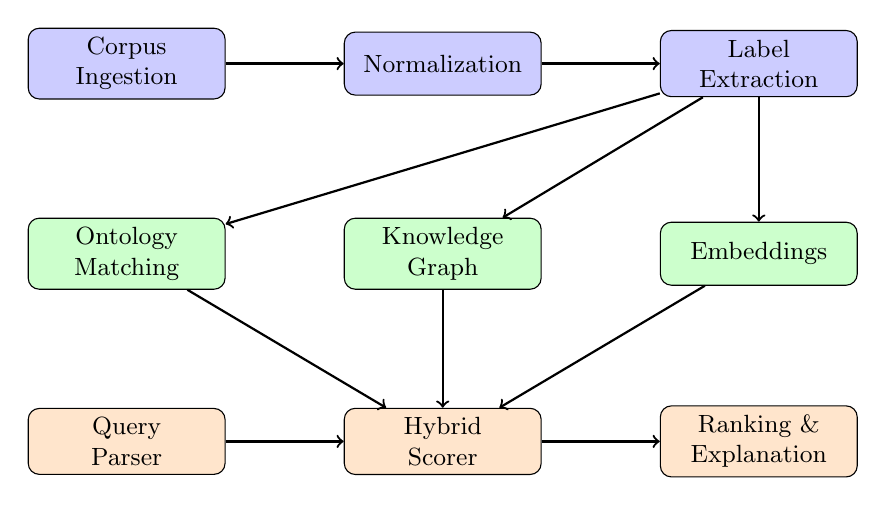
\begin{tikzpicture}[
    node distance=1.5cm,
    box/.style={rectangle, draw, rounded corners, minimum width=2.5cm, minimum height=0.8cm, align=center, font=\small},
    arrow/.style={->, thick}
]
    % Data layer
    \node[box, fill=blue!20] (corpus) {Corpus\\Ingestion};
    \node[box, fill=blue!20, right=of corpus] (normalize) {Normalization};
    \node[box, fill=blue!20, right=of normalize] (extract) {Label\\Extraction};

    % Knowledge layer
    \node[box, fill=green!20, below=of corpus] (ontology) {Ontology\\Matching};
    \node[box, fill=green!20, right=of ontology] (graph) {Knowledge\\Graph};
    \node[box, fill=green!20, right=of graph] (embed) {Embeddings};

    % Search layer
    \node[box, fill=orange!20, below=of ontology] (parse) {Query\\Parser};
    \node[box, fill=orange!20, right=of parse] (score) {Hybrid\\Scorer};
    \node[box, fill=orange!20, right=of score] (rank) {Ranking \&\\Explanation};

    % Arrows
    \draw[arrow] (corpus) -- (normalize);
    \draw[arrow] (normalize) -- (extract);
    \draw[arrow] (extract) -- (ontology);
    \draw[arrow] (extract) -- (graph);
    \draw[arrow] (extract) -- (embed);
    \draw[arrow] (ontology) -- (score);
    \draw[arrow] (graph) -- (score);
    \draw[arrow] (embed) -- (score);
    \draw[arrow] (parse) -- (score);
    \draw[arrow] (score) -- (rank);
\end{tikzpicture}
\caption{Neural Search Module Architecture}
\end{figure}

% ============================================================================
% SECTION 10: FUTURE DIRECTIONS
% ============================================================================
\section{Future Directions}
\label{sec:future}

\subsection{Sparse + Dense Hybrid Retrieval}

Implement BM25-based candidate generation with RRF fusion:
\begin{equation}
    \text{candidates} = \RRF(\BM_{\text{field}}(\cdot, \query), \text{Dense}(\cdot, \query), \text{Graph}(\cdot, \query))
\end{equation}

\subsection{Metapath-Based Explanations}

Enhance graph reasoning with explicit metapath templates and confidence-weighted path scoring:
\begin{equation}
    S_{\text{metapath}}(d, \query) = \sum_{\mathcal{P} \in \text{templates}(\query)} w_\mathcal{P} \cdot \max_{\text{path} \in \mathcal{P}(d)} \confidence(\text{path})
\end{equation}

\subsection{Learned-to-Rank Integration}

After sufficient human relevance labels, train calibrated rerankers:
\begin{equation}
    \score_{\text{learned}}(d, \query) = f_\theta\left(\mathbf{x}_{d,\query}\right)
\end{equation}
where $\mathbf{x}_{d,\query}$ is the feature vector and $f_\theta$ is learned (e.g., LambdaMART, neural ranker).

\subsection{Real Graph Proximity — Completed v0.9}

The $s_9$ graph proximity dimension was implemented in v0.9. When a \texttt{KnowledgeGraph} is available, PathSim is computed live:
\begin{equation}
    s_9(C_q, C_d) = \text{PathSim}_{\mathcal{P}}(\text{id}(C_q), \text{id}(C_d) \mid \graph)
\end{equation}

\subsection{Neural Signature Similarity (Phase 4)}

The $s_{10}$ dimension is a fixed placeholder ($0.0$). Phase 4 will extract neural population signatures directly from NWB/BIDS data:
\begin{equation}
    s_{10}(C_q, C_d) = \cos\!\left(\text{Extractor}(\text{NWB}(C_d)),\, \text{Extractor}(\text{NWB}(C_q))\right)
\end{equation}

\subsection{Human-Labeled Benchmark Calibration}

The v0.9 seed benchmark contains 49 human-assigned pairs spanning 7 intents (expanded from 30 in v0.8). The target for v1.1 is 200+ pairs to enable:
\begin{itemize}
    \item Calibrated usefulness score distributions
    \item Learned reranker training ($f_\theta$) on feature vectors
    \item Statistical significance testing across ablation variants
\end{itemize}

% ============================================================================
% SECTION 11: CONCLUSION
% ============================================================================
\section{Conclusion}
\label{sec:conclusion}

Neural Search represents a principled approach to scientific dataset discovery that goes beyond generic document retrieval. By formalizing datasets as structured experimental objects, grounding search in ontological knowledge, propagating provenance through typed graphs, and maintaining interpretable scoring, the system enables researchers to find reusable experimental contexts rather than merely similar text.

The mathematical foundations---spanning information retrieval theory, knowledge graph theory, representation learning, and evaluation methodology---provide a rigorous substrate for continued development. The current benchmark results (76.7\% P@5, 0.950 MRR, 0.937 NDCG@10) demonstrate the viability of the approach, while the architecture supports progressive enhancement toward larger corpora, learned ranking, and neural signature search.

The key insight remains: neuroscience search should retrieve reusable experimental contexts, not just documents. Neural Search makes this principle computationally tractable.

% ============================================================================
% REFERENCES
% ============================================================================
\bibliographystyle{plainnat}
\begin{thebibliography}{10}

\bibitem[Cormack et~al.(2009)]{cormack2009reciprocal}
Cormack, G.~V., Clarke, C.~L., and Buettcher, S.
\newblock Reciprocal rank fusion outperforms condorcet and individual rank learning methods.
\newblock In \emph{Proceedings of SIGIR}, pages 758--759, 2009.

\bibitem[Robertson and Zaragoza(2009)]{robertson2009probabilistic}
Robertson, S. and Zaragoza, H.
\newblock The probabilistic relevance framework: BM25 and beyond.
\newblock \emph{Foundations and Trends in Information Retrieval}, 3(4):333--389, 2009.

\bibitem[Salton et~al.(1975)]{salton1975vector}
Salton, G., Wong, A., and Yang, C.~S.
\newblock A vector space model for automatic indexing.
\newblock \emph{Communications of the ACM}, 18(11):613--620, 1975.

\bibitem[Sun et~al.(2011)]{sun2011pathsim}
Sun, Y., Han, J., Yan, X., Yu, P.~S., and Wu, T.
\newblock PathSim: Meta path-based top-k similarity search in heterogeneous information networks.
\newblock \emph{Proceedings of the VLDB Endowment}, 4(11):992--1003, 2011.

\bibitem[Karpukhin et~al.(2020)]{karpukhin2020dense}
Karpukhin, V., O\u{g}uz, B., Min, S., Lewis, P., Wu, L., Edunov, S., Chen, D., and Yih, W.-t.
\newblock Dense passage retrieval for open-domain question answering.
\newblock In \emph{Proceedings of EMNLP}, pages 6769--6781, 2020.

\bibitem[Bordes et~al.(2013)]{bordes2013translating}
Bordes, A., Usunier, N., Garcia-Duran, A., Weston, J., and Yakhnenko, O.
\newblock Translating embeddings for modeling multi-relational data.
\newblock In \emph{Advances in Neural Information Processing Systems}, pages 2787--2795, 2013.

\bibitem[J{\"a}rvelin and Kek{\"a}l{\"a}inen(2002)]{jarvelin2002cumulated}
J{\"a}rvelin, K. and Kek{\"a}l{\"a}inen, J.
\newblock Cumulated gain-based evaluation of IR techniques.
\newblock \emph{ACM Transactions on Information Systems}, 20(4):422--446, 2002.

\bibitem[Guo et~al.(2017)]{guo2017calibration}
Guo, C., Pleiss, G., Sun, Y., and Weinberger, K.~Q.
\newblock On calibration of modern neural networks.
\newblock In \emph{Proceedings of ICML}, pages 1321--1330, 2017.

\bibitem[Rubin{\'e}n et~al.(2024)]{rubinen2024dandi}
Rubi{\'e}n, D.~A., et~al.
\newblock The DANDI Archive: A platform for sharing standardized neurophysiology datasets.
\newblock \emph{Scientific Data}, 2024.

\bibitem[Markiewicz et~al.(2021)]{markiewicz2021openneuro}
Markiewicz, C.~J., et~al.
\newblock The OpenNeuro resource for sharing of neuroscience data.
\newblock \emph{eLife}, 10:e71774, 2021.

\end{thebibliography}

% ============================================================================
% APPENDIX
% ============================================================================
\appendix

\section{Algorithm Pseudocode}
\label{app:algorithms}

\begin{algorithm}
\caption{Neural Search Hybrid Retrieval}
\begin{algorithmic}[1]
\Procedure{Search}{$\query, \text{corpus}, \text{config}$}
    \State $\text{intent} \gets \Call{ClassifyIntent}{\query}$
    \State $\mathbf{w} \gets \Call{GetWeights}{\text{intent}, \text{config}}$
    \State $\text{parsed} \gets \Call{ParseQuery}{\query}$
    \State $\text{candidates} \gets \Call{GenerateCandidates}{\text{parsed}, \text{corpus}}$
    \State $\text{candidates} \gets \Call{FilterHardNegatives}{\text{candidates}, \text{parsed}}$
    \For{$d \in \text{candidates}$}
        \State $\text{scores}[d] \gets \Call{ComputeHybridScore}{d, \text{parsed}, \mathbf{w}}$
        \State $\text{explanations}[d] \gets \Call{GenerateExplanation}{d, \text{parsed}}$
    \EndFor
    \State $\text{ranked} \gets \Call{Sort}{\text{candidates}, \text{scores}}$
    \State \Return $\text{ranked}, \text{explanations}$
\EndProcedure
\end{algorithmic}
\end{algorithm}

\begin{algorithm}
\caption{BM25 Field-Weighted Scoring}
\begin{algorithmic}[1]
\Procedure{BM25Field}{$d, \query, \text{fields}, \mathbf{w}_f$}
    \State $\text{score} \gets 0$
    \For{$f \in \text{fields}$}
        \State $\text{score}_f \gets 0$
        \For{$t \in \query$}
            \State $\text{tf} \gets \Call{TermFreq}{t, d_f}$
            \State $\text{idf} \gets \Call{InverseDocFreq}{t}$
            \State $\text{len\_norm} \gets 1 - b + b \cdot |d_f| / \text{avgdl}_f$
            \State $\text{score}_f \gets \text{score}_f + \text{idf} \cdot \frac{\text{tf} \cdot (k_1 + 1)}{\text{tf} + k_1 \cdot \text{len\_norm}}$
        \EndFor
        \State $\text{score} \gets \text{score} + w_f \cdot \text{score}_f$
    \EndFor
    \State \Return $\text{score}$
\EndProcedure
\end{algorithmic}
\end{algorithm}

\begin{algorithm}
\caption{Reciprocal Rank Fusion}
\begin{algorithmic}[1]
\Procedure{RRF}{$\text{ranked\_lists}, k$}
    \State $\text{scores} \gets \{\}$
    \For{$R \in \text{ranked\_lists}$}
        \For{$i, d \in \Call{Enumerate}{R}$}
            \State $\text{scores}[d] \gets \text{scores}[d] + \frac{1}{k + i + 1}$
        \EndFor
    \EndFor
    \State \Return $\Call{SortByValue}{\text{scores}}$
\EndProcedure
\end{algorithmic}
\end{algorithm}

\section{Graph Schema Definition}
\label{app:schema}

\begin{lstlisting}[language=Python, caption=Knowledge Graph Schema (Pydantic)]
class NodeType(str, Enum):
    DATASET = "dataset"
    PAPER = "paper"
    TASK = "task"
    MODALITY = "modality"
    SPECIES = "species"
    REGION = "region"
    EVENT = "event"
    ANALYSIS = "analysis"
    STANDARD = "standard"
    REQUIREMENT = "requirement"

class EdgeType(str, Enum):
    HAS_TASK = "has_task"
    HAS_MODALITY = "has_modality"
    RECORDS_REGION = "records_region"
    HAS_SPECIES = "has_species"
    HAS_EVENT = "has_event"
    USES_STANDARD = "uses_standard"
    SUPPORTS_ANALYSIS = "supports_analysis"
    REQUIRES = "requires"
    LINKED_TO_PAPER = "linked_to_paper"
    SIMILAR_TO = "similar_to"

class GraphEvidence(BaseModel):
    source_type: str
    source_id: str
    source_field: Optional[str]
    evidence_text: Optional[str]
    extractor: str
    version: str
    confidence: float  # [0, 1]

class KnowledgeGraphNode(BaseModel):
    id: str
    node_type: NodeType
    label: str
    properties: Dict[str, Any]
    evidence: List[GraphEvidence]

class KnowledgeGraphEdge(BaseModel):
    id: str
    source: str
    target: str
    edge_type: EdgeType
    confidence: float
    evidence: List[GraphEvidence]
\end{lstlisting}

\end{document}
